\documentclass[10pt]{beamer}
\setbeameroption{show only notes}

\usetheme[progressbar=foot]{metropolis}
\makeatletter
\usepackage[caption=false]{subfig}
\usepackage{float}
\usepackage{textgreek}
\usepackage{mhchem}
\newlength\beamerleftmargin
\setlength\beamerleftmargin{\Gm@lmargin}
\usepackage[absolute,overlay]{textpos}
\usepackage{appendixnumberbeamer}
\setbeamertemplate{section in toc}[sections numbered]
\setbeamertemplate{subsection in toc}[subsections numbered]
\usepackage{booktabs}
\usepackage[scale=2]{ccicons}
\definecolor{utred}{RGB}{204,0,0}
\definecolor{utgray}{RGB}{128,128,128}
\usepackage{tikz}
\usepackage{graphicx}
\usepackage{pgfplots}
\usepackage{caption}
\captionsetup[figure]{labelformat=empty}
\setbeamertemplate{subsection in toc}
{\leavevmode\leftskip=2em\rlap{\hskip-2em$\quad$\inserttocsectionnumber.\inserttocsubsectionnumber}$\quad$\inserttocsubsection\par}
%%%%%%
\usepgfplotslibrary{dateplot}

\usepackage{xspace}
\newcommand{\themename}{\textbf{\textsc{metropolis}}\xspace}

\title{The Physicochemical Hydrodynamics of Vascular Plants}
\subtitle{A.D. Stroock, V.V. Pagay, M.A. Zwieniecki, N.M. Holbrook}
\date{\today}
\author{Andrew Watson}
\institute{University of Utah}
% \titlegraphic{\hfill\includegraphics[height=1.5cm]{logo.pdf}}

\setbeamercolor{progress bar in head/foot}{fg=utred,bg=utgray}
\setbeamercolor{progress bar in section page}{fg=utred,bg=utgray}
\setbeamercolor{progress bar in title separator}{fg=utgray,bg=black}
\setbeamercolor{frametitle}{bg=utred, fg=white}
\setbeamercolor{block title alerted}{fg=utred}
\setbeamercolor{alerted text}{fg = utred}
\setlength{\metropolis@titleseparator@linewidth}{1.5pt}
\setlength{\metropolis@progressonsectionpage@linewidth}{1.5pt}
\setlength{\metropolis@progressinheadfoot@linewidth}{3pt}
\setlength{\metropolis@progressonsectionpage@linewidth}{1.5pt}

\setbeamerfont{bibliography item}{size=\scriptsize}
\setbeamerfont{bibliography entry author}{size=\scriptsize}
\setbeamerfont{bibliography entry title}{size=\scriptsize}
\setbeamerfont{bibliography entry location}{size=\scriptsize}
\setbeamerfont{bibliography entry note}{size=\scriptsize}

\setlength{\fboxsep}{0pt}
\setlength{\fboxrule}{.25pt}

\newcommand{\vect}[1]{\boldsymbol{\mathbf{#1}}}
\newcommand{\tn}{\textnormal}

\begin{document}

\maketitle

\addtobeamertemplate{frametitle}{}{%
\begin{tikzpicture}[remember picture,overlay]
  \node[anchor=north east,yshift=2pt] at (current page.north east)
  {\includegraphics[height=0.7cm]{ulogo@2x.png}};
\end{tikzpicture}}

\section{Introduction to Transport in Plants}

\begin{frame}{Photosynthesis}
  \begin{columns}
    \begin{column}{.59\textwidth}
      \begin{itemize}
        \note[item]{A useful place to begin talking about plant
          biology is to compare plants with animals, because people
          are usually more familiar with animal biology than with
          plant biology}
        \note[item]{This review starts out by talking about
          photosynthesis, which seems like a good place to start
          because plants' ability to do photosynthesis is probably
          their single most defining characteristic}
      \item Photosynthesis may be the most defining characteristic of
        plants
        \note[item]{Partly as a consequence of photosynthesis,
          plants are adapted for extracting diffuse, but ubiquitous
          molecules and energy from their environment, and so they are
          adapted to maximize surface area. By contrast, animals are
          adapted for motion, because they (we) consume concentrated
          and patchily distributed food.}
      \item Plants maximize surface area to extract diffuse,
        ubiquitous resources
      \item \ce{6CO2 + 6H2O ->[light] C6H12O6 + 6O2}
      \item Photosynthesis happens (mostly) in the leaves---that's
        where the light is!
      \item Water is extracted from the soil, and has to be delivered
        to the leaves, where it is consumed by photosynthesis and lost
        to the atmosphere
      \item Pores on the leaves allow \ce{CO2} to enter, but also
        allow water to evaporate
      \end{itemize}
    \end{column}
    \begin{column}{.4\textwidth}
      \vfill
      \includegraphics[width=\textwidth]{trillium}
      \vfill
    \end{column}
  \end{columns}
\end{frame}

\begin{frame}{Plant Vascular System}
  \begin{columns}
    \begin{column}{.49\textwidth}
      \begin{itemize}
        \note[item]{The vascular system in plants serves the same
          function as the vascular system in animals: transport stuff
          throughout the body. However the mechanisms for this
          transport, and the architecture of the vascular system are
          completely different.}
      \item Vascular system---transport stuff through the body
      \item In animals, the heart \emph{pushes} fluid through vessels
      \item In plants, leaves \emph{pull} fluid up from the roots
        (``negative pressure,'' i.e. below atmospheric pressure)
      \item Two vessel types:
        \begin{enumerate}
        \item Xylem---transport water and nutrients up from the soil
          to leaves
        \item Phloem---transport sugars from leaves to the rest of the
          plant
        \end{enumerate}
      \end{itemize}
    \end{column}
    \begin{column}{.49\textwidth}
      \vfill
      \includegraphics[width=\textwidth]{plant_vasculature}
      \vfill
    \end{column}
  \end{columns}
\end{frame}

\begin{frame}{Plant Vessel Structure}
  \begin{columns}
    \begin{column}{.49\textwidth}
      \begin{itemize}
        \note[item]{Our vasculature is basically a network of pipes,
          where cells form the vessel walls, and fluid is conducted
          through the empty space in the middle. In plants, the fluid
          is conducted \emph{through} specialized cells. (Refer to the
        figure on the right). }
      \item Fluid is conducted \emph{through} specialized cells,
        instead of ``pipes'' with a large intercellular space
        \note[item]{It is generous to even call the cells of the xylem
          cells}
      \item Specialized xylem cells are dead cells; basically just an
        empty cell wall and cell membrane (diameters up to 0.5 mm!)
      \item Phloem cells are living, but their volume is still mostly
        dedicated to transporting sap
      \end{itemize}
    \end{column}
    \begin{column}{.49\textwidth}
      \vfill
      \includegraphics[width=\textwidth]{plant_vasculature}
      \vfill
    \end{column}
  \end{columns}
\end{frame}

\begin{frame}{Negative Pressure and Cavitation}
  \begin{center}
    \includegraphics[width=.7\textwidth]{fig3_crop}
  \end{center}
  \begin{itemize}
    \note[item]{I will talk more about this a little later, but
      because the water in the xylem has a pressure below atmospheric
      pressure, it is vulnerable to spreading air bubbles}
  \item The segmented vessels provide a safeguard against
    spreading air bubbles, which interrupt the flow
    \note[item]{I guess in the plant/animal analogy, air bubbles are
      like clots, but that's a \emph{bit} of a strained comparison}
  \item Pores in the membranes between xylem cells allow them to
    support a pressure difference between adjacent cells
  \item Young-Laplace law: $\displaystyle{\Delta P_\tn{max} =
      \frac{4\gamma \cos{\theta_r}}{d_p}}$ ($\gamma$---water surface
    tension) 
    \note[item]{Young-Laplace law gives an upper bound on the pore
      diameter for a given pressure difference, if the plant wants to
      stop the air bubble from spreading to adjacent cells.}
  \item In extreme cases, fluid pressure can drop to -10 MPa
    $\implies d_p < 22 \, \tn{nm}$ (max occurs at $\theta_r = 0$)
    \note[item]{In plants where the pressure drop is less extreme,
      pore diameters can be larger. They don't mention this in the
      paper, but it seems as least plausible to me that larger pores
      would offer less resistance to fluid flow, and would be
      preferred in pressure regimes that allow it.}
  \end{itemize}
\end{frame}

\section{Transport in the Xylem and Phloem}

\begin{frame}{Water Potential}
  \begin{itemize}
    \note[item]{Botanists use the potential energy of water to
      track the flow of water through plants, which they call
      ``water potential,'' but to me it makes the most sense to
      think of it as pressure. Water potential has the same units
      as pressure, and it works like any other potential field:
      stuff flows from areas of high potential to areas of low
      potential.}
  \item Water potential ($\Psi_w$) is the chemical potential of
    water, normalized so pure water at $P_0$ has $\Psi_w = 0$
  \item $\displaystyle{\Psi_{w, l} = \underbrace{(P -
        P_0)}_{\tn{pressure component}} - \underbrace{RT
        C_s}_{\tn{osmotic potential}} + \underbrace{\rho_l g
        z}_{\tn{gravity component}} +
      \underbrace{\Psi_\tn{matrix}}_{\tn{matrix effects}}}$ 
  \item Usually $\Psi_\tn{matrix} < 0$, i.e. the matrix effects
    tend to be stabilizing
    \note[item]{The matrix effects are due to the interaction of
      water with a matrix like tissue or soil; it tends to have a
      stabilizing effect}
  \item $\displaystyle{\Psi_{w, v} = \underbrace{\frac{RT}{v_l}
        \ln\left(\frac{p_v}{p_\tn{sat}} \right)}_\tn{humidity} +
      \rho_l g z}$
  \item $P_0$---atmospheric pressure, $C_s$---concentration of
    solutes, $p_v$ \& $p_\tn{sat}$---vapor pressure and saturation
    vapor pressure
  \end{itemize}
\end{frame}

\begin{frame}{Water Potential}
  \vfill
  \begin{center}
    \includegraphics[width=.7\textwidth]{water_potential}
  \end{center}
  \note[item]{As I mentioned before, as water is consumed by
    photosynthesis and evaporates from the leaves, it pulls up water
    through the xylem from the roots. This is totally passive, the
    plant doesn't need to expend any energy to do this; the water is
    always flowing down its potential gradient.}
  \note[item]{The transport of fluid through the phloem is active;
    sugars are pumped into phloem cells at the leaf, which pulls water
    in from the xylem, generating a positive pressure and forcing the
    water-sugar solution down the phloem.}
  \vfill
\end{frame}

\begin{frame}{Pressure and Solute Concentraction without Flow}
  \begin{columns}
    \begin{column}{.69\textwidth}
      \begin{itemize}
      \item Assume stomata in the leaves are closed, and there is no
        solute loading in the phloem
      \item At equilibrium, the water potential in the xylem $\Psi_X$
        and phloem $\Psi_P$ are equal to $\Psi_\tn{soil}$
      \item In the xylem, $C_s = 0$ and $\Psi_{X, \tn{matrix}} = 0$,
        so
        \begin{multline*}
          \Psi_X = (P - P_0) - RTC_s + \rho_l g z + \Psi_{X,
            \tn{matrix}} \\
          \implies \Psi_\tn{soil} = (P - P_0) + \rho_l g z \\
          \implies P_X(z) = P_0 - \rho_l g z + \Psi_soil
        \end{multline*}
      \item Pressure drops linearly in the xylem with height; where
        $P_X(z) < p_\tn{sat}$, the water is superheated and prone to
        boiling
      \end{itemize}
    \end{column}
    \begin{column}{.29\textwidth}
      \vfill
      \includegraphics[width=\textwidth]{water_potential_c}
      \vfill
    \end{column}
  \end{columns}
\end{frame}

\begin{frame}{Pressure and Solute Concentraction without Flow}
  \begin{columns}
    \begin{column}{.69\textwidth}
      \begin{itemize}
      \item In the phloem, 
        \begin{multline*}
          \Psi_P = (P - P_0) - RTC_s + \rho_l g z + \Psi_{X,
            \tn{matrix}} \\
          \implies \Psi_\tn{soil} = (P - P_0) - RT C_{s, P} + \rho_l g
          z \\ 
          \implies C_{s, P} (z) = \frac{1}{RT}(\Delta P_P + \rho_l g z
          - \Psi_soil) 
        \end{multline*}
        \note[item]{This illustrates how plants can regulate the
          pressure in their phloem cells by transporting solutes
          in/out of the phloem cells}
      \item Plants can regulate the pressure in their phloem cells by
        altering solute concentration
      \end{itemize}
    \end{column}
    \begin{column}{.29\textwidth}
      \vfill
      \includegraphics[width=\textwidth]{water_potential_c}
      \vfill
    \end{column}
  \end{columns}
\end{frame}

\section{Coupled Flows}

\begin{frame}{Coupled Flows}
  \begin{columns}
    \begin{column}{.49\textwidth}
      \begin{align*}
        \Delta \Psi_{s-a} = \Delta P_X + Q_{w, \tn{trans}} (R_{X, r} +
        R_{X, l}) - \rho_l g h \\
        \Delta P_X = R_X (Q_{w, \tn{trans}} + Q_{w, P}) + \rho_l g h
        \\
        \Delta P_P = R_P Q_{w, P} - \rho_l g h\\
        RT \Delta C_{s, P} = R_{P, \tn{tot}} Q_{w, P} + \Delta P_X -
        \rho_l g h \\
        \Delta C_{s, P} = \frac{Q_\tn{sol}}{v_l Q_{w, P}}
      \end{align*}
      \note[item]{$h$ is the height of the plant}
      \begin{itemize}
      \item The $R$'s are resistances, $Q$'s are (molar) flow rates,
        $P$'s are pressures
      \end{itemize}
    \end{column}
    \begin{column}{.49\textwidth}
      \vfill
      \begin{center}
        \includegraphics[width=.6\textwidth]{water_potential_a}
      \end{center}
      \vfill
    \end{column}
  \end{columns}
\end{frame}

\begin{frame}{Coupled Flows}
  \begin{itemize}
  \item These equations can be solved for the two flow rates:
    \begin{align*}
      \left[\frac{R_{P, \tn{tot}}}{R_X} + \frac{R_{X, r} + R_{X,
      l}}{R_{X, \tn{tot}}}\right] Q_{w, P}^2 + \left[\frac{\Delta
      \Psi_{s-a}}{R_{X, \tn{tot}}}\right] Q_{w, P} -
      \frac{Q_\tn{sol}}{R_X} \frac{RT}{v_l} = 0 \\
      Q_{w, \tn{trans}} = \frac{\Delta \Psi_{s-a} - R_X Q_{w,
      P}}{R_{X, \tn{tot}}}
    \end{align*}
  \item $Q_{w,P}$ depends on a combination of the resistances, the
    difference in water potential between the soil and atmosphere, and
    the loading rate of solute into the phloem.
    \note[item]{In particular, the flow rate through the phloem
      increases with increasing solute loading rate}
  \item $Q_{w, \tn{trans}}$ depends on the resistance in the xylem,
    the difference in water potential, and the flow rate through the
    phloem
  \end{itemize}
\end{frame}

\begin{frame}{Coupled Flows: Nighttime and Solute Loading}
  \begin{columns}
    \begin{column}{.69\textwidth}
      \begin{itemize}
      \item Special case: closed stomata ($R_{X, l} \rightarrow
        \infty$) and $Q_sol > 0$.
      \item In this limit $Q_{w, \tn{trans}} = 0$ and,
        \begin{align*}
          Q_{w, P} = \left( \frac{RT / v_l}{R_{P, \tn{tot}} + R_X}
          Q_\tn{sol} \right)^{1/2} \\
          \Delta C_{s, P} = \left(\frac{R_{P, \tn{tot}} + R_X}{v_l RT}
          Q_\tn{sol} \right)^{1/2}
        \end{align*}
      \item Assuming $R_{P, \tn{tot}}$ and $R_X \sim \tn{height}$,
        then $Q_{w, P} \sim \tn{height}^{-1/2}$
      \item Measurements of phloem pressure within small plants are
        consistent with the predictions of this theory, but not for
        larger plants and trees
      \end{itemize}
    \end{column}
    \begin{column}{.29\textwidth}
      \vfill
      \includegraphics[width=\textwidth]{water_potential_d}
      \vfill
    \end{column}
  \end{columns}
\end{frame}

\begin{frame}{Leaf Size in Trees}
  \begin{itemize}
  \item It is observed that shorter trees have greater variability in
    leaf length than tall trees
  \item Jensen \& Zwieniecki (2013) present an argument based on
    energy flux mediated by the movement of sugar molecules
  \item $E = k c u$; $E$---energy flux, $u$---flow speed of phloem
    sap, $c$---concentration of sugar, $k$---energy per sugar molecule
  \item Assume the plant has 3 parts, with associated resistances: a
    source (leaves), a stem, and a sink (roots, fruit, etc.)
  \item $R_\tn{source} = 1 / (2\pi r l L_p)$; $l$---leaf length,
    $r$---radius of phloem tube, $L_p$---permeability of phloem
    membrane
    \note[item]{R source is the resistance to the transport of water
      into phloem vessels}
  \item $R_\tn{stem} = 8 \eta h / (\pi r^4)$; $\eta$---viscosity of
    sap, $h$---tree height
    \note[item]{R stem assumes the phloem in the stem acts as a
      cylindrical tube with radius $r$}
  \item $R_\tn{sink} = 1 / (2\pi r s L_p)$; $s$---length of sink
    region
  \item Assume $s \gg r$, then $R_\tn{sink} \ll R_\tn{source}$ and
    \begin{equation*}
      u = \frac{1}{\pi r^2} \frac{\Delta p}{R_\tn{source} +
        R_\tn{stem}} = \frac{2 r^2 L_p l}{r^3 + 16 \eta L_p l h}
      \Delta p
    \end{equation*}
  \end{itemize}
\end{frame}

\begin{frame}{Leaf Size in Trees}
  \begin{equation*}
    u = \frac{1}{\pi r^2} \frac{\Delta p}{R_\tn{source} +
      R_\tn{stem}} = \frac{2 r^2 L_p l}{r^3 + 16 \eta L_p l h}
    \Delta p
  \end{equation*}
  \begin{itemize}
  \item $u$ decreases monotonically with increasing $h$, due to added
    resistance in the stem
  \item If $l$ is small, then $u$ increases linearly with $l$, however
    as $l \rightarrow \infty$, $u$ approaches an asymptote
    \note[item]{Diminishing returns}
  \end{itemize}
  \includegraphics[width=\textwidth]{energy_constraints}
\end{frame}

\begin{frame}{Leaf Size in Trees}
  \begin{columns}
    \begin{column}{.49\textwidth}
      \begin{itemize}
      \item
        $\displaystyle{l_\tn{max} = \frac{1}{16} \frac{r^3}{\tau L_p
            \eta} \frac{1}{h}}$
      \item
        $\displaystyle{l_\tn{min} = \frac{1}{16} \frac{r^3}{L_p \eta}
          \frac{1}{h_\tn{max} - h}}$
      \item They fit these two functions to the points shown in red
        and blue
      \end{itemize}
    \end{column}
    
    \begin{column}{.49\textwidth}
      \vfill
      \includegraphics[width=\textwidth]{tree_height}
      \vfill
    \end{column}
  \end{columns}
\end{frame}

% \begin{frame}{Priming experiments}
%   \begin{figure}
%     \centering
%     \setlength{\fboxsep}{0pt}
%     \setlength{\fboxrule}{.25pt}
%     \fbox{\includegraphics[width=.75\textwidth]{expt-sideview}}
%     \caption{Side view of the priming microfluidic
%       chambers. Eichinger, Ph.D. dissertation, 2016}
%     \label{fig:flow-chambers}
%   \end{figure}

%   \begin{itemize}
%   \item Nonlocal effects---experiments from
%     Proteins-Polymers-Interfaces group led by Dr. Hlady
%     \note[item] {Brief background: they are generally interested in
%     designing materials that can be implanted into bloodstream without
%     triggering clotting \& immune responses}
%   \item Platelets can transiently bind to agonists without firmly
%     adhering, and be primed for full downstream activation
%     \note[item] {Perhaps not surprising, but not considered or
%     quantified in traditional materials tests}
%   \end{itemize}
% \end{frame}

% \begin{frame}{Priming Experiments}
%   \begin{figure}
%     \centering
%     \fbox{\includegraphics[width=.75\textwidth]{expt-sideview}}
%     \caption{Side view of the priming microfluidic
%       chambers. Eichinger, Ph.D. dissertation, 2016}
%     \label{fig:flow-chambers}
%   \end{figure}

%   \begin{itemize}
%   \item Some results: more primed platelets adhere in the capture
%     region than unprimed, primed platelets have higher levels of
%     P-selectin expression and active
%     \textalpha\textsubscript{IIb}\textbeta\textsubscript{3} 
%   \item Rolling data extracted: average velocities, step sizes, pause times
%   \end{itemize}
% \end{frame}

% \begin{frame}{Adhesive dynamics models}
%   \note[item] {Rolling specifically refers to the combined physical and
%   chemical process of platelet motion in blood near a vessel wall, and
%   binding kinetics of platelet receptors with immobilized agonists}
% \begin{columns}
%   \begin{column}{.5\textwidth}
%     \begin{itemize}
%     \item Components of Adhesive Dynamics models:
%       \begin{itemize}
%       \item Random bond formation and breaking (tracking individual
%         receptors and bonds)
%       \item FSI: Stokes flow around a rigid body (spheres in
%         traditional AD, ellipsoids in platelet AD)
%       \end{itemize}
%     \item Bond-level kinetics $\rightarrow$ cell-level behavior
%     \end{itemize}
%   \end{column}

%   \begin{column}{.5\textwidth}
%     \begin{figure}
%       \centering
%       \fbox{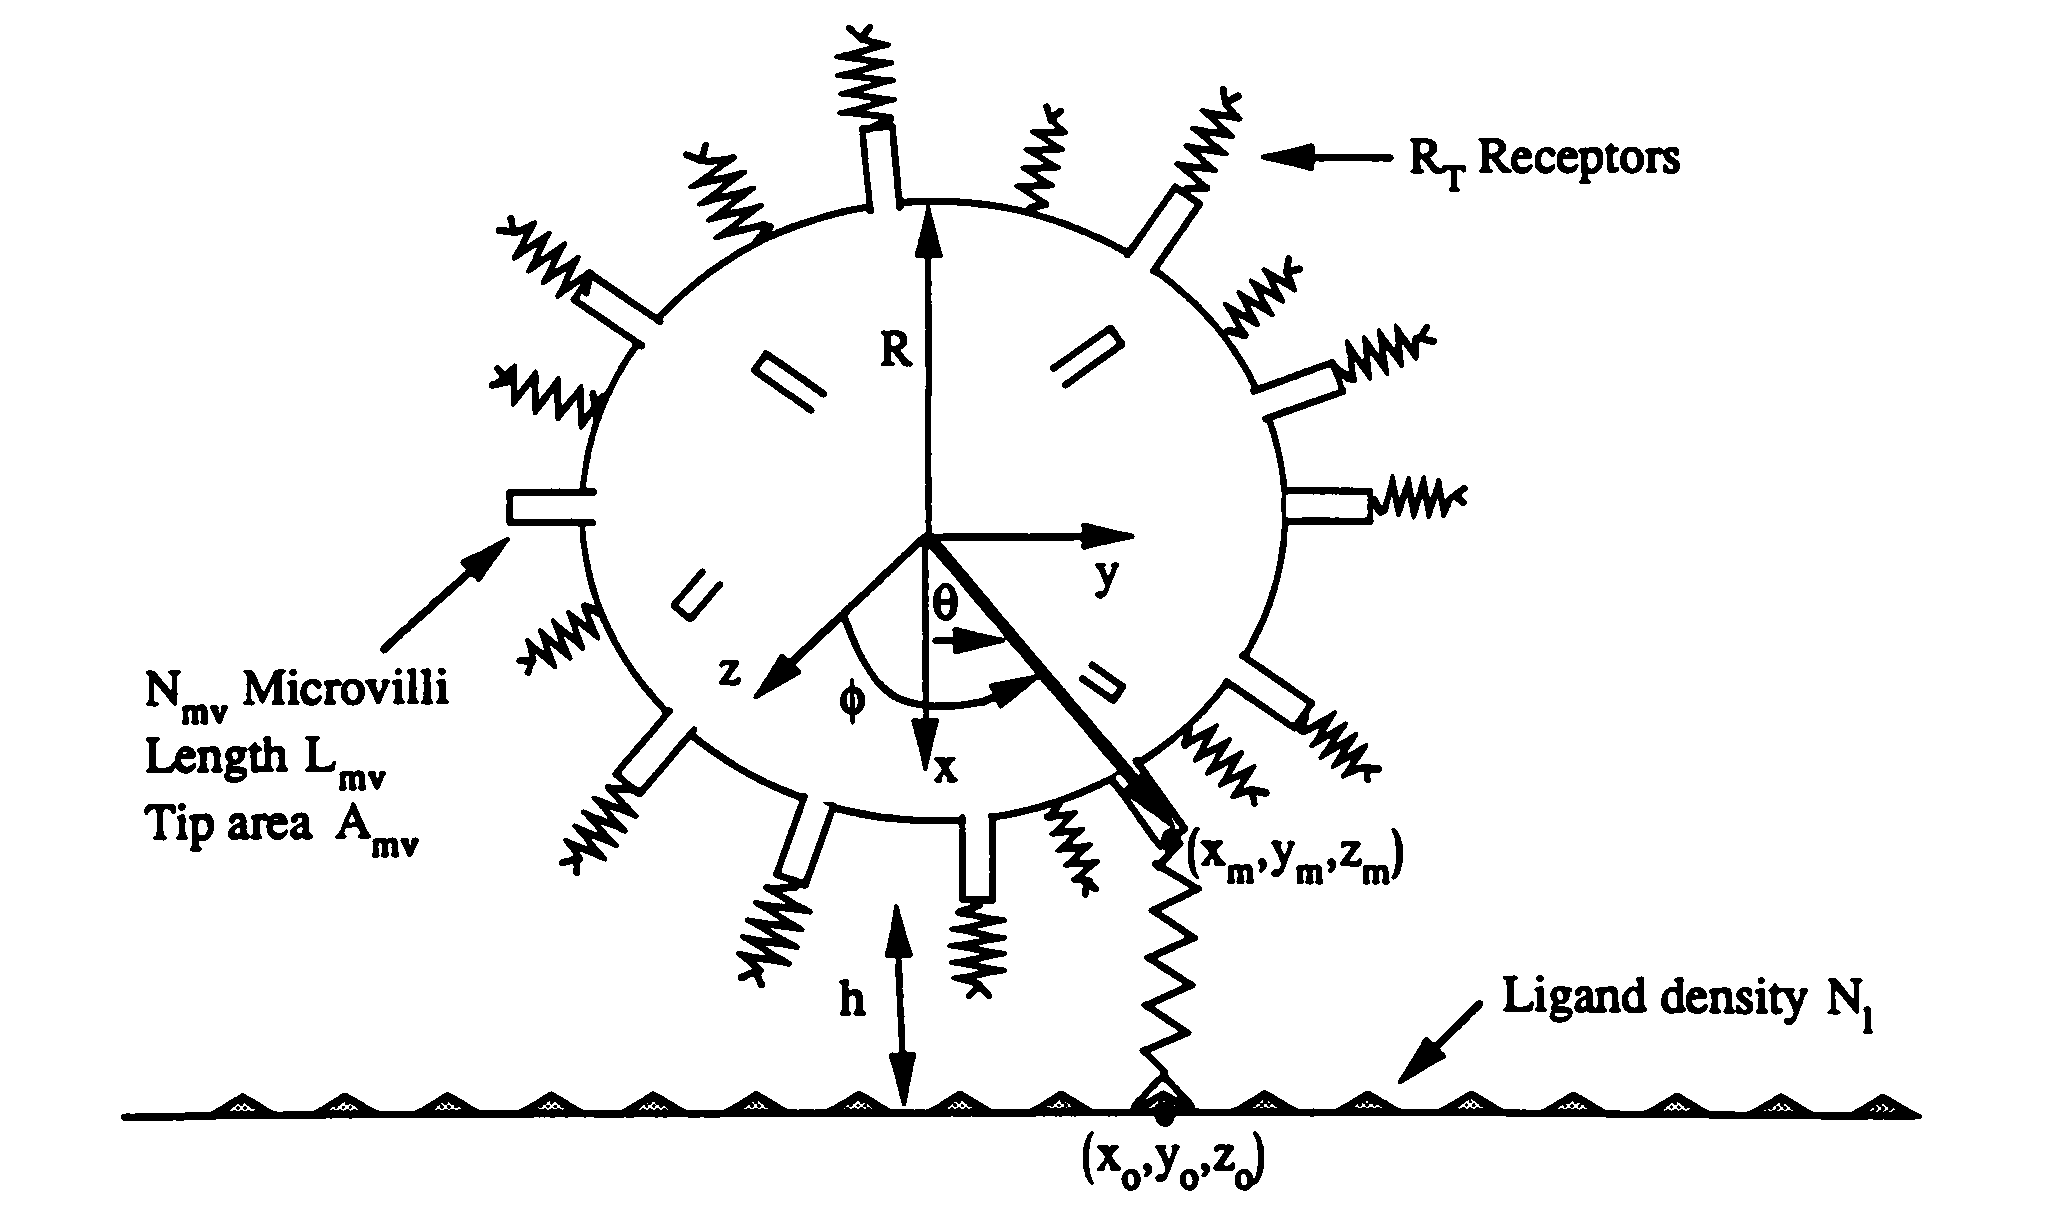
\includegraphics[width=\textwidth]{hammer92scr}}
%       \caption{Geometry of a leukocyte AD model. From Hammer \&
%         Apte, 1992}
%       \label{fig:hammer-diagram}
%     \end{figure}
%   \end{column}
% \end{columns}
% \note[item] {We want to find parameters that give realistic rolling
%   behavior in the 3D model, and tweak binding parameters to model the
%   effects of priming on rolling behavior}
% \end{frame}

% \section{Numerics \& Model}

% \begin{frame}{Definitions and domain}
%   \begin{columns}
%     \begin{column}{.5\textwidth}
%       \begin{itemize}
%       \item Fluid domain is the upper half space where $x > 0$
%       \item Wall is the plane at $x = 0$
%       \item Background flow: $\vect{v}^\infty = \gamma x \vect{e}_z$
%       \item Platelet: ellipsoid with axes $1.5 \times 1.5 \times 0.5$,
%         center of mass at $\vect{x}_c$, orientation vector
%         $\vect{e}_m$
%         \note[item] {$\vect{e}_m$ is a unit vector in the direction of
%           the minor axis. This is sufficient to define the
%           orientation, since the platelet is rotationally symmetric
%           about the minor axis} 
%       \item Fluid satisfies steady Stokes equations with no-slip BCs
%         on the wall and platelet surface:
%         \begin{align*}
%           &\Delta \vect{v} = \nabla P, \, \nabla \cdot
%             \vect{v} = 0 \\
%           &\vect{v}(\vect{x})|_{\partial P} = \vect{U} +
%             \vect{\Omega} \times \vect{x} \\
%           &\vect{v}|_{x = 0} = 0, \, \vect{v}(\vect{x})|_{\|\vect{x}\|
%             \rightarrow \infty} \rightarrow \vect{v}^\infty(\vect{x}) 
%         \end{align*}
%         \note[item] {$\vect{U}$ is the translational velocity of the
%           platelet, and $\vect{\Omega}$ is the angular velocity of the
%           platelet. Next, talk about platelet motion.}
%       \end{itemize}
%     \end{column}

%     \begin{column}{.4\textwidth}
%       \begin{figure}
%         \centering
%         \subfloat{\fbox{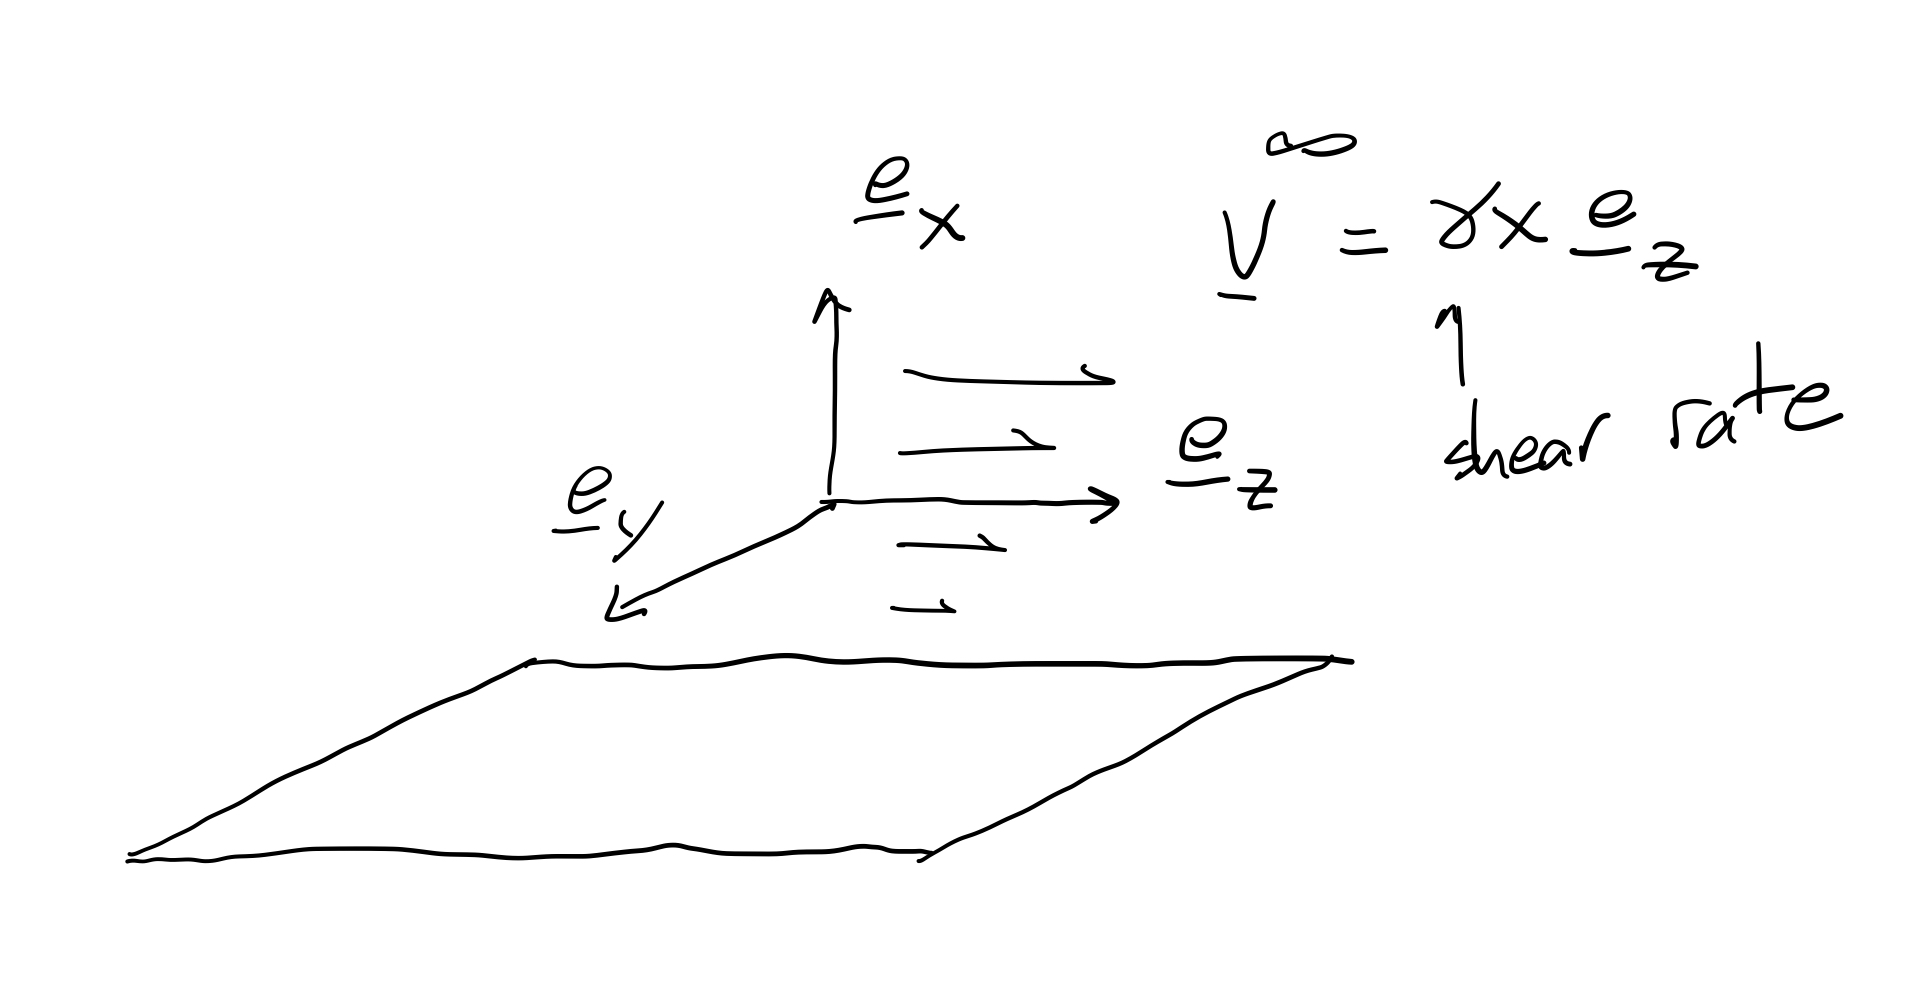
\includegraphics[width=\textwidth]{axes}}} \\
%         \subfloat{\fbox{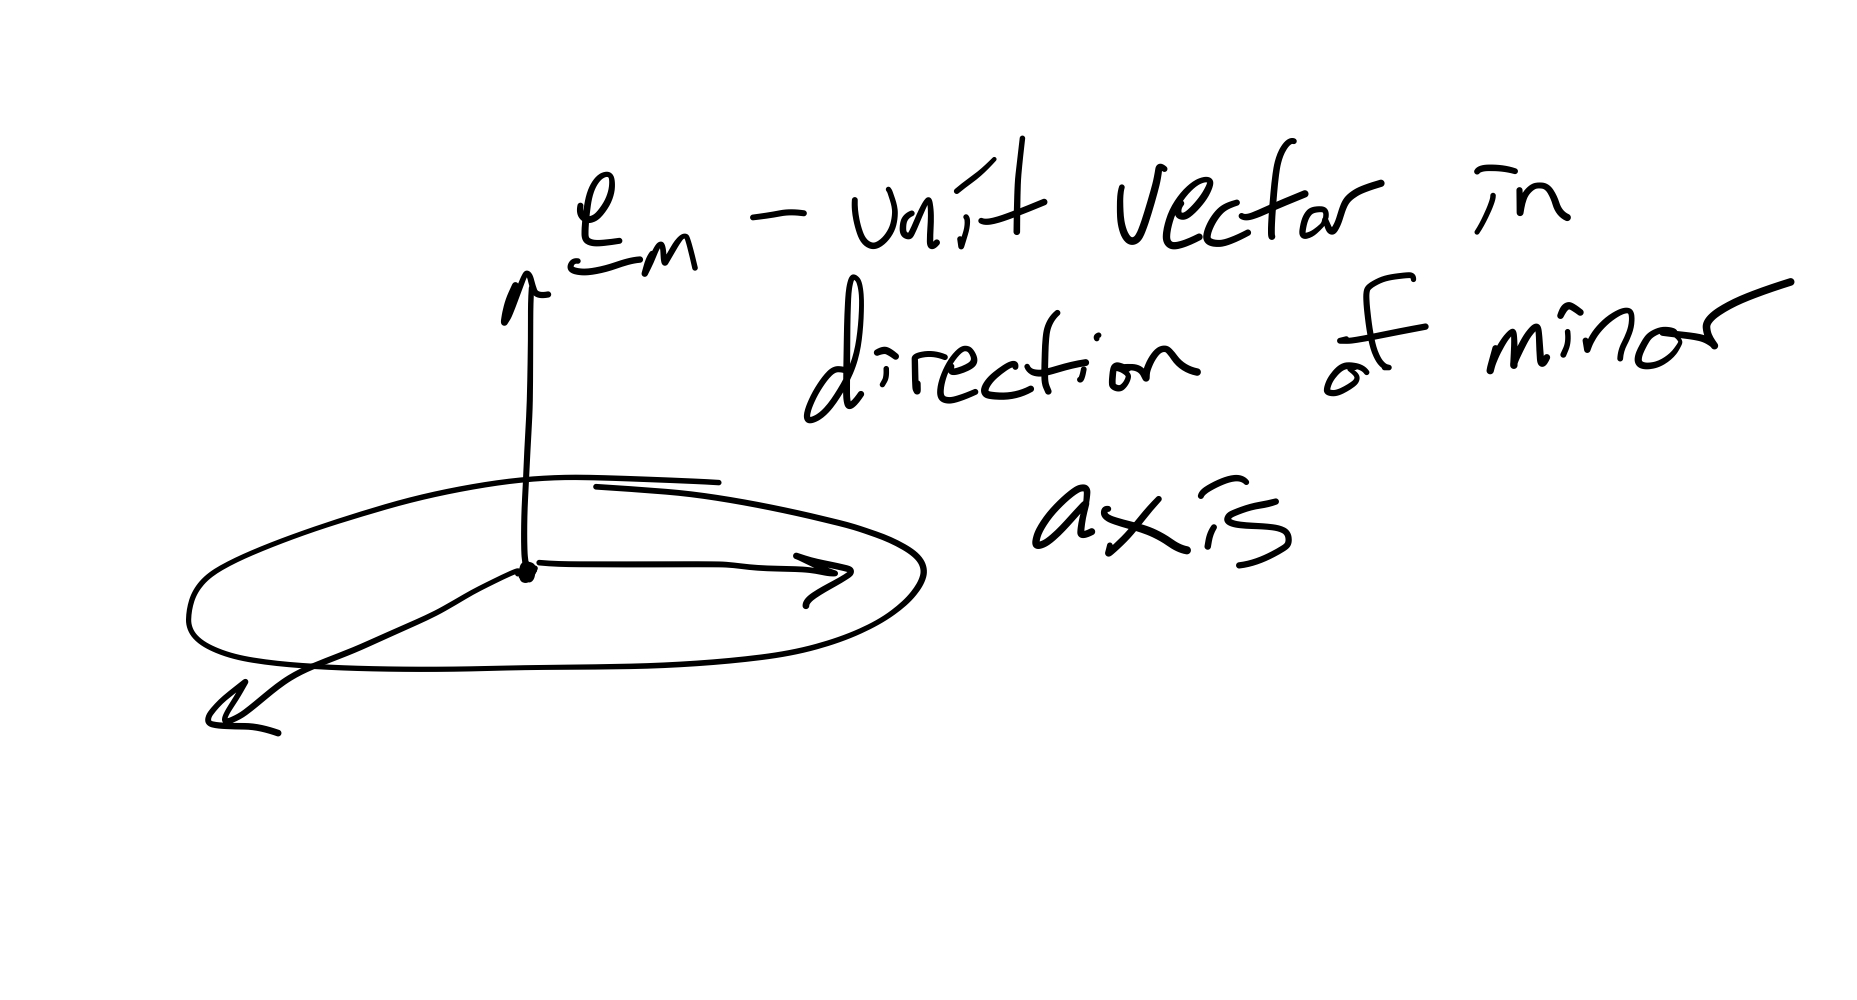
\includegraphics[width=\textwidth]{reference}}} 
%         \caption{Sketch of the axes and orientation of the ellipsoid}
%         \label{fig:orient-sketch}
%       \end{figure}
%     \end{column}
%   \end{columns}
% \end{frame}

% \begin{frame}{Platelet motion}
%   \begin{itemize}
%     \note[item] {Equations of rigid body motion}
%   \item Equations of motion:
%     \begin{equation*}
%       \frac{d\vect{x}_c}{dt} = \vect{U}(\vect{x}_c, \vect{e}_m), \,
%       \frac{d\vect{e}_m}{dt} = \vect{\Omega}(\vect{x}_c, \vect{e}_m)
%       \times \vect{e}_m
%     \end{equation*}
%     \note[item] {Of course, evaluating the RHS is the hard part}
%   \item $\vect{U}$ and $\vect{\Omega}$ are found by balancing forces
%     and torques on the platelet body.
%   \item Define $\vect{F}^h$ and $\vect{T}^h$ to be the hydrodynamic
%     forces on the platelet, and $\vect{F}^o$ and $\vect{T}^o$ to be
%     other forces/torques acting on the platelet
%     \note[item] {Most significantly bond forces, however past adhesive
%       dynamics simulations have included other chemical forces acting
%       on the platelet as well.}
%   \item Given a velocity field $\vect{v}$, then
%     \begin{align*}
%       \vect{F}^h &= \int_{\partial P} \underline{\underline{\sigma}}
%                    \cdot \vect{n} ds(\vect{x}) \\
%       \vect{T}^h &= \int_{\partial P} (\vect{x} - \vect{x}_c) \times
%                    \underline{\underline{\sigma}} \cdot \vect{n}
%                    ds(\vect{x}) 
%     \end{align*}
%     \note[item] {$\sigma$ is the stress tensor of $\vect{v}$}
%   \item If we assume $\vect{F}^o$ and $\vect{T}^o$ are known given a
%     position and orientation, then we ``just'' need to find $\vect{U}$
%     and $\vect{\Omega}$ such that $\vect{F}^h + \vect{F}^o = 0$
%     \note[item] {This is hard because we need $\vect{U}$ and
%       $\vect{\Omega}$ to solve Stokes' equations, but these are
%       unknown at the start of a time step.}
%   \end{itemize}
% \end{frame}

% \begin{frame}{Solving for $\vect{U}$ and $\vect{\Omega}$}
%   \begin{itemize}
%   \item We can decompose $\vect{F}^h$ into a drag force $\vect{F}^d$
%     generated by a platelet moving through a stationary background
%     flow, and $\vect{F}^s$ which represents the drag force on a
%     stationary platelet in a background shear flow
%     \note[item] {And same for the torques}
%   \item Because of the linearity of Stokes flow, there is a linear
%     relationship between $(\vect{F}^d, \vect{T}^d)$ and $(\vect{U},
%     \vect{\Omega})$: 
%     \begin{align*}
%       \vect{F}^d &= -(\mathcal{T} \vect{U} + \mathcal{P}
%       \vect{\Omega}) \\
%       \vect{T}^d &= -(\mathcal{P}^T \vect{U} + \mathcal{R}
%       \vect{\Omega}) 
%     \end{align*}
%   \item The resistance matrices $\mathcal{T}$, $\mathcal{P}$, and
%     $\mathcal{R}$ depend only on the shape of the body, and its
%     position and orientation
%   \item The resistance matrices can be found by solving 6 different
%     Stokes flow problems---three translations and three
%     rotations
%   \item $\vect{F}^s$ and $\vect{T}^s$ are found with 7th solve, where
%     the platelet is stationary and the background flow is a shear flow
%     \note[item] {These solves are done with regularized Stokeslets}
%   \end{itemize}
% \end{frame}

% \begin{frame}{Regularized Stokeslets}
%   \note[item] {I think I've already exceeded the number of math slides
%     acceptable in this presentation}
%   \begin{itemize}
%   \item In the method of regularized Stokeslets, approximate point
%     forces are placed on a structure (a surface, thin filament, or
%     even discrete points)
%   \item Analytic representations of fluid flow have been derived for
%     these approximate point forces, and can be summed together to find
%     the resulting fluid flow
%   \item Often (and in my case), there is a desired \emph{velocity} at
%     certain points, and the Stokeslets strengths must be solved for
%   \end{itemize}
% \end{frame}

% \begin{frame}{Binding and Unbinding}
%   \begin{itemize}
%   \item One simple model of length dependent binding and unbinding
%     comes from Dembo et. al. (1988):
%     \begin{align*}
%       k_f(r) &= k_f^0 \exp \left(\frac{-\sigma_\tn{ts} (r -
%                \lambda)^2}{2k_B T} \right) \\
%       k_d(r) &= k_d^0 \exp \left(\frac{(\sigma - \sigma_\tn{ts})(r -
%                \lambda)^2}{2k_B T} \right) \\
%     \end{align*}
%     where $r = \| \vect{x}_\tn{receptor} - \vect{x}_\tn{ligand}
%     \|$, $\lambda$ is the rest length of the receptor-ligand bond, and
%     $\sigma$ and $\sigma_\tn{ts}$ are Hookean spring constants
%   \item If $\sigma < \sigma_\tn{ts}$, then the bonds are slip bonds
%   \item Some later AD models use catch-slip bond kinetics, which
%     requires a more complicated model of binding and unbinding
%     \note[item] {Receptors distributed uniformly over the surface of
%       the platelet, and ligands distributed on the wall}
%   \item From these rates, we can find probabilities of bonds
%     forming/breaking within a time step
%   \end{itemize}
% \end{frame}

% \begin{frame}{Current and Near-Future Work}
%   \begin{itemize}
%   \item I am working on adding stochastic binding and unbinding to the
%     model
%   \item Find parameter values that give reasonable rolling behavior
%     \note[item] {These experiments are likely too expensive to do true
%     parameter fitting; just want behavior that is close to observations}
%   \item Run experiments with ``unprimed'' and ``primed'' (through
%     changing binding parameters) platelets and assemble statistics
%   \end{itemize}
% \end{frame}

\end{document}
